\begin{frame}{$K^0$ Cross Section Calculation}
  \begin{tabular}{cc}
    \begin{minipage}{0.5\hsize}
      \begin{figure}
        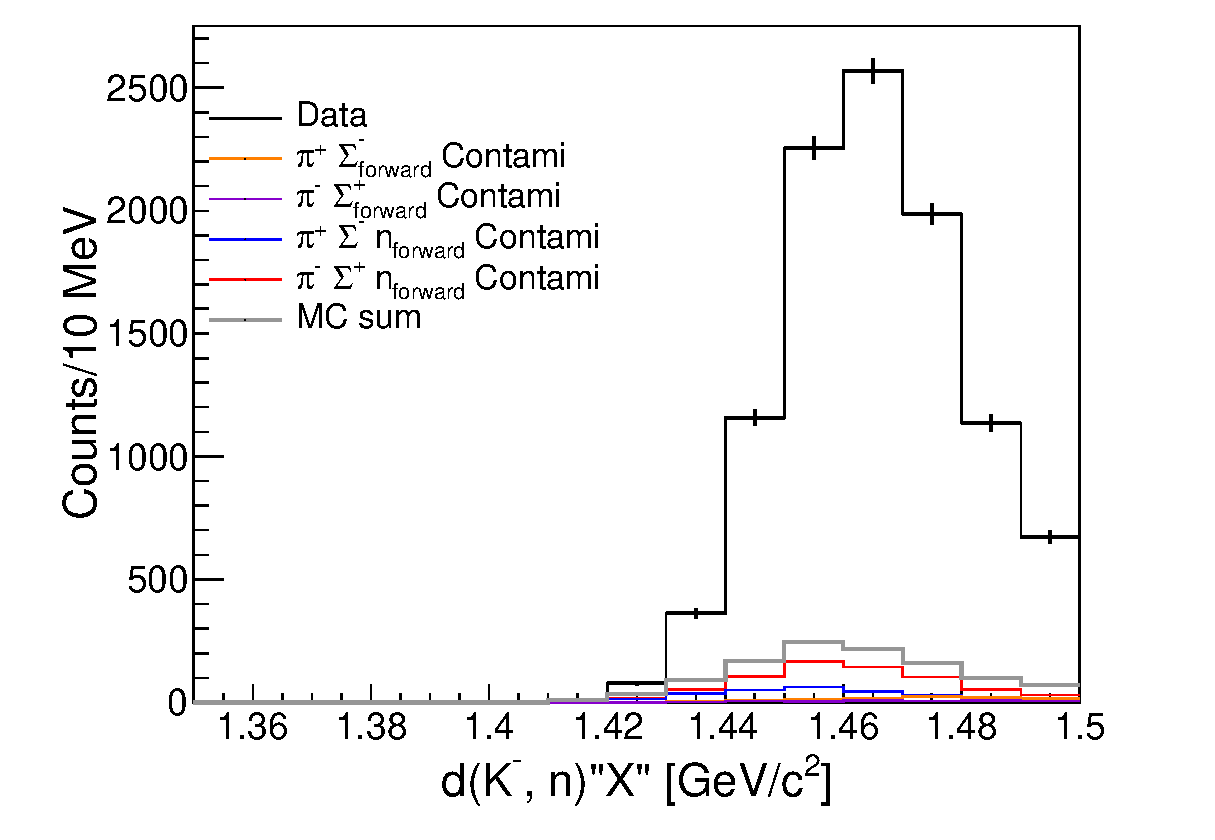
\includegraphics[width=5cm]{../pic/Run78/QE/KN_MM_wK0_tag.eps}
      \end{figure}
      \centering
      \vspace{-4mm}
      \scriptsize
      $K^0$ tagged events with background were estimated by MC template.
    \end{minipage}

    \begin{minipage}{0.5\hsize}
      \begin{figure}
        \scriptsize
        Acceptance about $\cos\theta_{K_0}$ vs $p_{K_0}$
        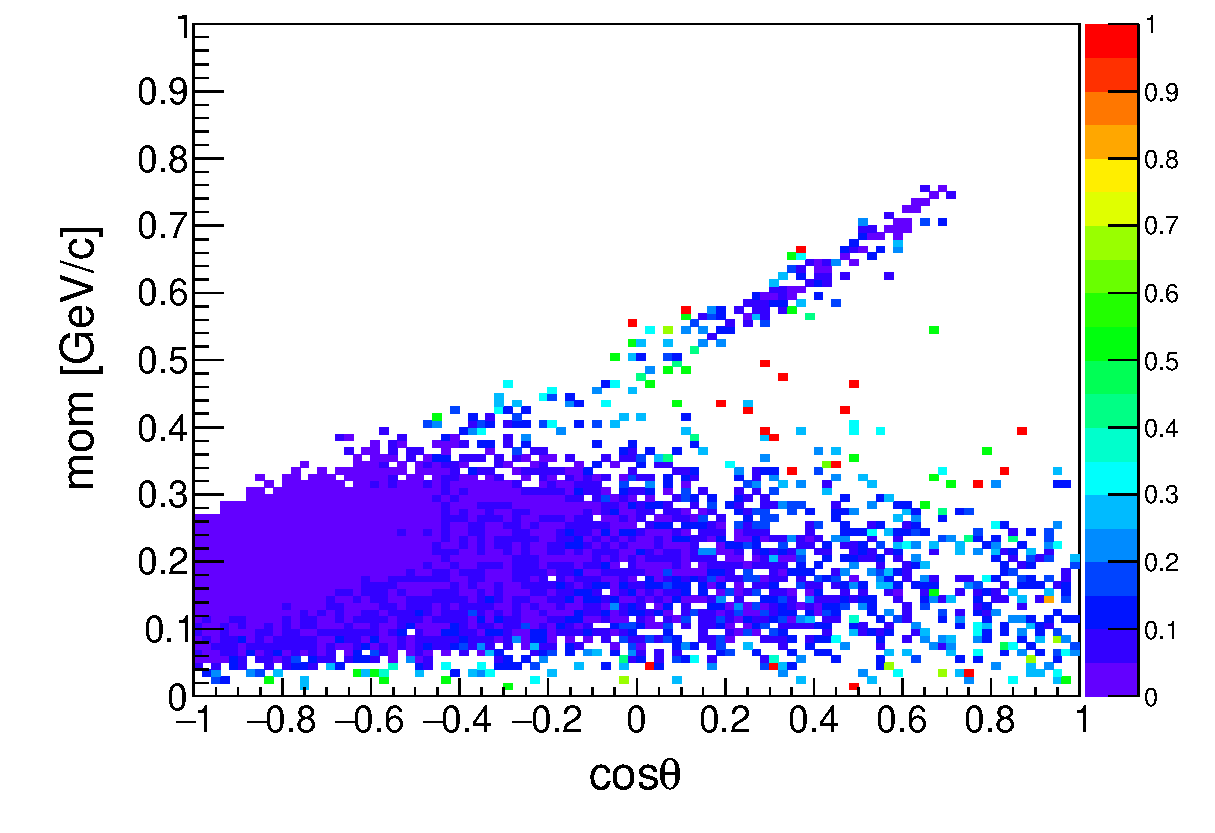
\includegraphics[width=5cm]{../pic/Run78/QE/K0_cos_mom_acc.eps}
      \end{figure}
      \centering
      \vspace{-4mm}
      \small
      $\frac{(\mbox{Analyzed events})}{(\mbox{Generated events})}$
    \end{minipage}
  \end{tabular}
  \begin{itemize}
  \item Convert mothod to Cross Section\\
    \footnotesize
    Calculation to CS was performed event-by-event using $K^0$ kinematics ($\cos\theta$, $p$).
    \begin{equation*}
      \frac{d^2\sigma}{d\Omega dM_{d(K^-, n)}}=F\times \sum M(\cos\theta, p)\times\frac{1}{A(\cos\theta, p)}
    \end{equation*}
  \end{itemize}
\end{frame}
